%% Document template source: LaTeX2e template for FEUP's Project FE-UP
%% Document template author: jlopes@fe.up.pt
%% Template adapted

%% A alterar: <--ALTERAR-->

\documentclass[11pt,a4paper]{report}

%% Macros ----------------------------------------------------------------------{{{1
\newcommand{\school}{Instituto Superior de Engenharia de Lisboa}
\newcommand{\degree}{Licenciatura em Engenharia Eletrotécnica, Telecomunicações e Computadores}
\newcommand{\projisel}{Projeto ISEL 2023/24 --- LEETC}
\newcommand{\projtitle}{RCp}
\newcommand{\projsubtitle}{Subtítulo do Trabalho}
\newcommand{\projteam}{Grupo LP-07}

%% Package ---------------------------------------------------------------------{{{1
\usepackage{graphicx}           % 
\usepackage[portuguese]{babel}  % [portuges]??
\usepackage{multicol}           % 
\usepackage{longtable}          % Tables continue in the next page
\usepackage{listings}           % Programming syntax

%importados e verificar
\usepackage[utf8]{inputenc}     % accents
\usepackage{color}
\usepackage[a4paper,left=25mm,right=25mm,top=25mm,bottom=25mm,headheight=6mm,footskip=12mm]{geometry}   % Document dimensions
\usepackage{lastpage}           % 
\usepackage{fancyhdr}           % Headers and footers
\usepackage{hyperref}           % Hyper references
\usepackage{chicago}            % Bibliography style


%verificar
\usepackage[T1]{fontenc}          % PS fonts
\usepackage{newtxtext,newtxmath}  % do not use CM fonts
\usepackage{amsmath}              % multi-line and other mathematical statements
\usepackage{setspace}             % setting the spacing between lines
\usepackage[normalem]{ulem}       % various types of underlining
\usepackage{caption}              % rotating captions, sideways captions, etc.
\usepackage{float}                % tables and figures in the multi-column environment 
\usepackage{subcaption}           % for subfigures and the like
\usepackage{multirow}             % tabular cells spanning multiple rows
\usepackage[table]{xcolor}        % driver-independent color extensions
\usepackage{lipsum}               % loren dummy text
\setlength{\marginparwidth}{2cm}  % todonotes' requirements
\usepackage{todonotes}            % todo's

%% my other macros, if needed
\newcommand{\windspt}{\textsf{WindsPT\/}}
\newcommand{\windscannerpt}{\emph{Windscanner.PT\/}}
\newcommand{\class}[1]{{\normalfont\slshape #1\/}}
\newcommand{\svg}{\class{SVG}}

%% my environments for infos
\newenvironment{info}[1]{\vspace*{6mm}\color{blue}[ \begin{em} #1}
                        {\vspace*{6mm}\end{em} ]}
\newenvironment{infoopt}[1]{\vspace*{6mm}\color{blue}[ \textbf{Elemento opcional.} \begin{em} #1}
                        {\vspace*{6mm}\end{em} ]}


%% Package settings ------------------------------------------------------------{{{1
\graphicspath{{./images/}}                          % {graphicx} - Images path
\selectlanguage{portuguese}                         % {babel} - Language portuguese
\setlength{\columnsep}{3cm}                         % {multicol} - Column spacement
\definecolor{engineering}{rgb}{0.549,0.176,0.098}   % {color}
\definecolor{cloudwhite}{cmyk}{0,0,0,0.025}         % {color}
\setlength{\parindent}{0em}                         % {geometry}
\setlength{\parskip}{1ex}                           % {geometry}
\lstdefinestyle{pythoncode}                         % {listings} - Python syntax
{
    keepspaces=true,
    numbersep=5pt,

    basicstyle=\footnotesize\ttfamily,
    keywordstyle=\bfseries,
    numbers=left,                                   % where to put the line-numbers
    numberstyle=\scriptsize\texttt,                 % the size of the fonts that are used for the line-numbers
    stepnumber=1,                                   % the step between two line-numbers. If it's 1 each line will be numbered
    numbersep=8pt,                                  % how far the line-numbers are from the code
    frame=tb,
    float=htb,
    aboveskip=8mm,
    belowskip=4mm,
    backgroundcolor=\color{cloudwhite},             
    showspaces=false,                               % show spaces adding particular underscores
    showstringspaces=false,                         % underline spaces within strings
    showtabs=false,                                 % show tabs within strings adding particular underscores
    tabsize=2,                                      % sets default tabsize to 2 spaces
    captionpos=b,                                   % sets the caption-position to bottom
    breaklines=true,                                % sets automatic line breaking
    breakatwhitespace=false,                        % sets if automatic breaks should only happen at whitespace
    escapeinside={\%*}{*)},                         % if you want to add a comment within your code
    morekeywords={*,var,template,new}               % if you want to add more keywords to the set
}
\fancyhf{}                                          % {fancyhdr} clear off all default fancyhdr headers and footers
\lfoot{\small{\emph{\projtitle, \projsubtitle}}}    % {fancyhdr}
\rfoot{\small{\thepage\ / \pageref{LastPage}}}      % {fancyhdr}
\pagestyle{fancy}                                   % {fancyhdr} apply the fancy header style
\renewcommand{\headrulewidth}{0.0pt}                % {fancyhdr} no head rule
\renewcommand{\footrulewidth}{0.4pt}                % {fancyhdr}
\hypersetup{                                        % {hyperref}
    plainpages=false,
    pdfpagelayout=SinglePage,
    bookmarksopen=false,
    bookmarksnumbered=true,
    breaklinks=true,
    linktocpage,
    colorlinks=true,
    linkcolor=engineering,
    urlcolor=engineering,
    filecolor=engineering,
    citecolor=engineering,
    allcolors=engineering
}

%\usepackage{comment}               % Permite criar um segmento de comentários (/begin{comment} [...] /end{comment})
%\usepackage{xcolor}                % Colorir texto (esta versão é mais flexível do que a {color})
%\usepackage{subcaption}            % Subcaptions para figuras
%\usepackage{fullpage}              % Utilizar página inteira

%% Document start --------------------------------------------------------------{{{1
\begin{document}
\pagenumbering{roman}\setcounter{page}{1}

%% Cover -----------------------------------------------------------------------{{{1
\begin{titlepage}
    \center

    \vspace*{-12mm}
    {\large \textbf{\textsc{\school}}}\\

    \vfill

    \includegraphics[width=62mm]{<--ALTERAR-->}
    
    \vfill
    
    {\huge \textbf{\projtitle}}\\[6mm]
    {\Large \textbf{\projsubtitle}}\\
    
    \vfill
    
    \includegraphics[width=52mm]{<--ALTERAR-->}
    
    \vfill
    
    {\Large \textbf{\projisel}}\\[12mm]
    
    {\Large \textbf{Coordenação}}\\[4mm]
    {\large Geral:  \hspace*{18mm}
            De curso: }\\[6mm]
    
    {\Large \textbf{\projteam}}\\[4mm]
    {\large Supervisor: \hspace*{12mm}
            Monitor: }\\[6mm]
    
    {\Large \textbf{Estudante}}\\[4mm]
    {\large Nuno Brito $<$A46948@alunos.isel.pt$>$ \hspace*{12mm}
    
    \renewcommand{\today}{<--ALTERAR-->}
    \today
    
\end{titlepage}

%% TOC -------------------------------------------------------------------------{{{1
\tableofcontents

%% List of figures -------------------------------------------------------------{{{1
\listoffigures
\addcontentsline{toc}{chapter}{Lista de figuras}


%% List of tables --------------------------------------------------------------{{{1
\listoftables
\addcontentsline{toc}{chapter}{Lista de tabelas}

%% Acronyms --------------------------------------------------------------------{{{1
\chapter*{Lista de acrónimos}
\addcontentsline{toc}{chapter}{Lista de acrónimos}

\begin{flushleft}
\begin{tabular}{l p{0.8\linewidth}}
    API     & Application Programming Interface\\
    GUI     & Graphical User Interface\\
    HTTP    & Hyper Text Transfer Protocol\\
    OS      & Operating System\\
    OSS     & openSUSE\\
    PHP     & PHP: Hypertext Preprocessor\\
    SSL     & Secure Sockets Layer\\
    TCP     & Transmission Control Protocol\\
    TLS     & Transport Layer Security\\
    TUI     & Terminal User Interface\\ % Not used yet
    UDP     & User Datagram Protocol\\
    VPN     & Virtual Private Network\\
    WWW     & World Wide Web\\
    XAMPP   & Cross-Platform, Apache, MySQL, PHP, and Perl
\end{tabular}
\end{flushleft}

%% Glossary --------------------------------------------------------------------{{{1
\chapter*{Glossário}
\addcontentsline{toc}{chapter}{Glossário}

\begin{description}
    \item[Operating system] \hfill \\
        A program that manages a computer's resources from software to hardware.
    \item[Browser] \hfill \\
        A browser is a internet navigation software. It comes in multiple flavours, nowadays the big three are Microsoft Edge, Mozilla Firefox and Google Chrome.
    \item[Windows] \hfill \\
        Microsoft's operating system. First released in 1985 as a Graphical User Interface (GUI) for MS-DOS, continued to evolve with it's latest version being 11.
    \item[Rolling release distribuition] \hfill \\
        A distribuition where it's software release cycle is more frequent than those of Long Term Support (LTS). It's up to the Linux-based distribuitor to guarantee
        the testing of a package.
        Due to it's nature, it's not recommended for server production environment.
    \item[openSUSE Tumbleweed] \hfill \\
        An openSUSE (OSS) is an open-source community driven Linux-based distribuition sponsored by SUSE Software Solutions. Tumbleweed is a rolling release version 
        allowing for up-to-date software releases.
    \item[Wireshark] \hfill \\
        Wireshark is a network protocol analyser software. Allows traffic capture between a computer and a network.
    \item[LibreWolf] \hfill \\
        An internet browser based on Mozilla's Firefox. It's primary purpose is to allow privacy, and with it comes security. It achieves this by removing telemetry and
        data collection.
    \item[XAMPP] \hfill \\
        A software package environment collection containing Apache2 webserver, MariaDB database, PHP and Perl.
    \item[Apache2] \hfill \\
        Text
    \item[Socket] \hfill \\
        Text
    \item[Python] \hfill \\
        Python is a high-level programming language, object-oriented.
    \item[Firewall] \hfill \\
        Text
    \item[VPN] \hfill \\
        Text
    \item[SSL] \hfill \\
        Text
    \item[] \hfill \\
        Text
    \item[] \hfill \\
        Text
    \item[] \hfill \\
        Text
    \item[] \hfill \\
        Text
    \item[] \hfill \\
        Text
    \item[] \hfill \\
        Text
    \item[] \hfill \\
        Text

\item[bash] \hfill \\
  Bash é uma \emph{shell Unix} e uma linguagem de comando escrita
  em 1989 por Brian Fox para o Projeto GNU como um substituto de
  software livre para a \emph{Bourne shell}.
\item[firewall] \hfill \\
  Em computação, uma \emph{firewall} é um sistema de segurança de rede
  que monitoriza e controla o tráfego de entrada e saída da rede
  com base em regras de segurança predeterminadas.
  Uma \emph{firewall} normalmente estabelece uma barreira entre uma
  rede confiável e uma rede não confiável, como a Internet.
\item[Glossário] \hfill \\
  Glossário é uma espécie de pequeno dicionário específico para
  palavras e expressões pouco conhecidas presentes num texto, seja
  por serem de natureza técnica, regional ou de outro idioma.
\end{description}

%% Chapter: introduction -------------------------------------------------------{{{1
\chapter{Introduction}
%% display headers & footers
\pagestyle{fancy}
%% main page numbers with arabic numerals
\pagenumbering{arabic}\setcounter{page}{1}



%% Chapter: project ------------------------------------------------------------{{{1
\chapter{Phase 1}
    \section{Milestones}
        \begin{itemize}
            \item Setup apache2 web server in localhost
            \item Access web server locally (http://127.0.0.1/)
            \item Access web server from a remote computer
            \item Use wireshark in a remote host to capture packages from the server
            \item Compare the HTTP headers sent by the client and the server
            \item Develop a simple barebones HTTP webclient
            \item Establish a TCP connection to the server
            \item Request the base webpage
        \end{itemize}
        
    \section{WebClient requirements}
        \begin{itemize}
            \item HTTP library forbidden
            \item Establish TCP connection using available sockets library - send/receive the HTTP request/reply
            \item Output HTTP reply to the user
            \item - Optional - act to the various HTTP replies
            \item Text-only application
        \end{itemize}

    \subsection{Software}
        \item Local server side
            \subitem Operating system: Windows 11 x64
            \subitem WebServer: XAMPP x64 8.2.12-0-VS16 for windows
        Disclaimer: the versions listed below might not be the latest, by present date, given the nature of rolling release distribuitions software updates.
        \item Client side
            \subitem Operating system: openSUSE Tumbleweed
            \subitem Browser: LibreWolf version 123.0-1
            \subitem Package monitor: Wireshark version 4.2.3 (Git commit b0da86c196d1).
    
    \subsection{Software install steps}
        Step-by-step instructions performed
        Xampp install
        wireshark install
        wireshark settings
        wireshark filters

        Webclient output
        Wireshark outputs browser
        Wireshark outputs webclient

        % Yo reduce the ammount of pictures! Or maybe side by side 
        Number one step is to install, start and configure XAMPP. Using the following \url{https://www.apachefriends.org/download.html}{link} we can choose our prefered
        method, for this project the portable version was the best choice since no installation was needed.
        After uncompressing our downloaded file, we can start the process.
        \begin{tabular}{ l r }
            The read me file available in the root directory states that
            we need to run \textit{setup_xampp} batch file first to populate the
            registry it's directory.                                        & 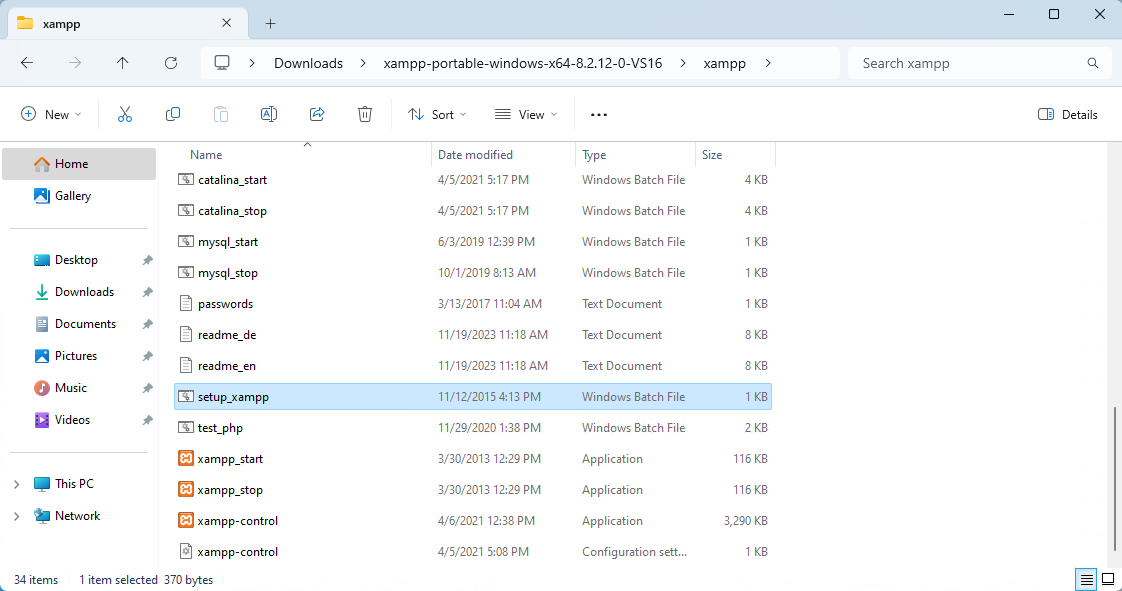
\includegraphics[scale=0.3]{install_xampp08} \\ % 0.3 scale!

            After completing, just press any button to continue.            & 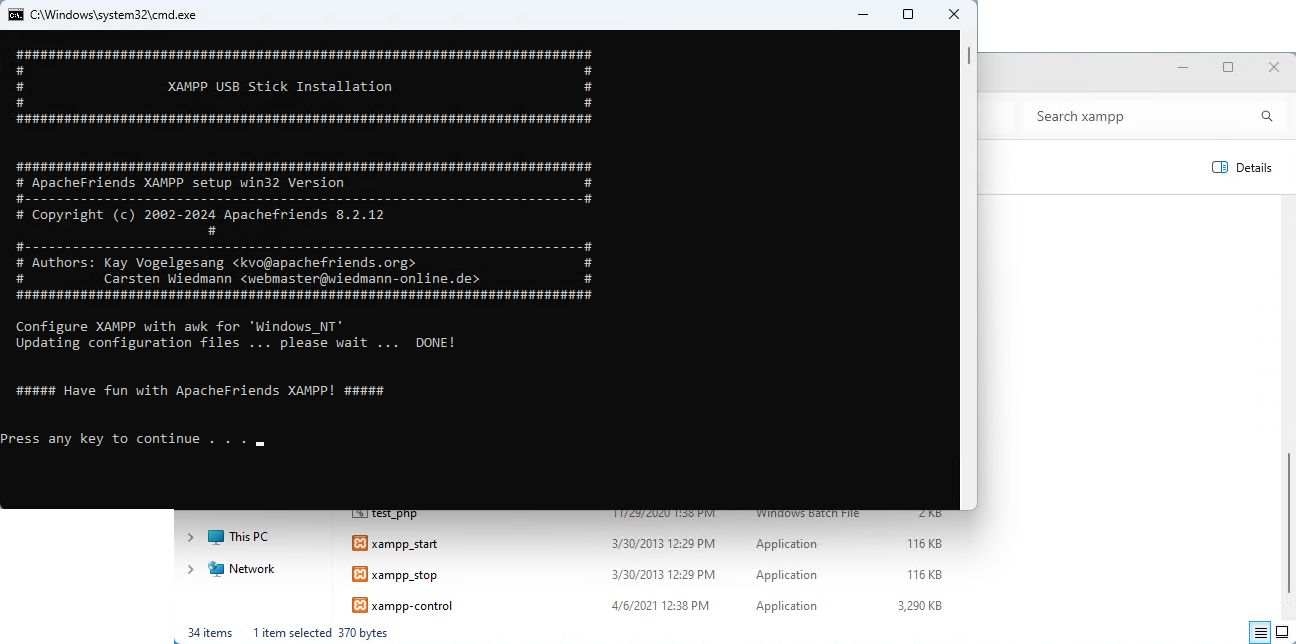
\includegraphics[scale=0.3]{install_xampp09} \\

            Next click in the \textit{xampp_start} executable, windows
            will prompt some firewall permissions which will gladly accept. & 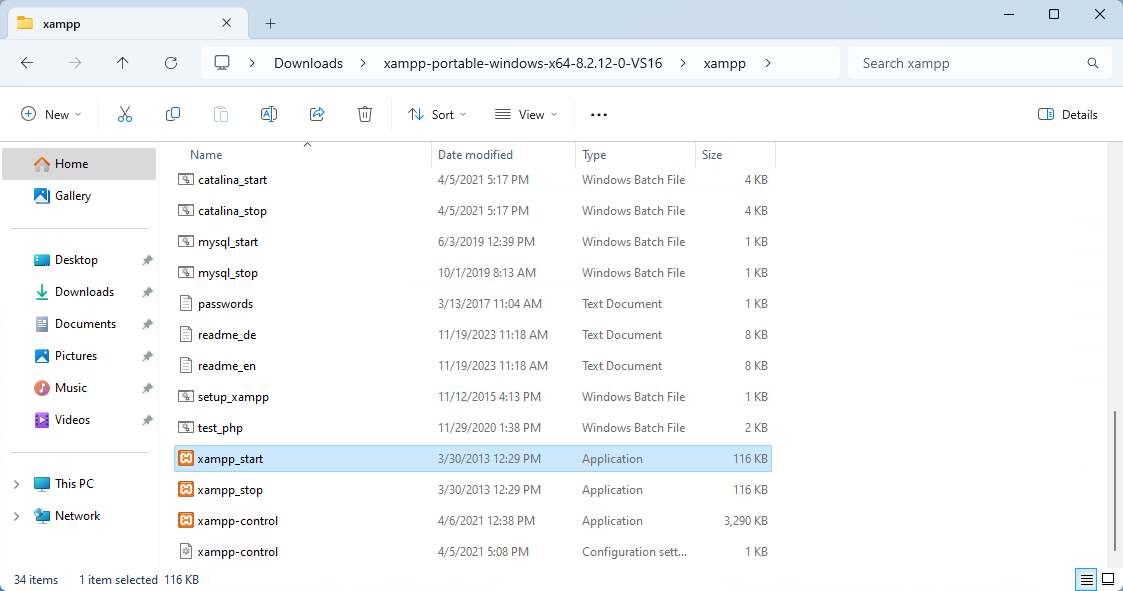
\includegraphics[scale=0.3]{install_xampp10} & 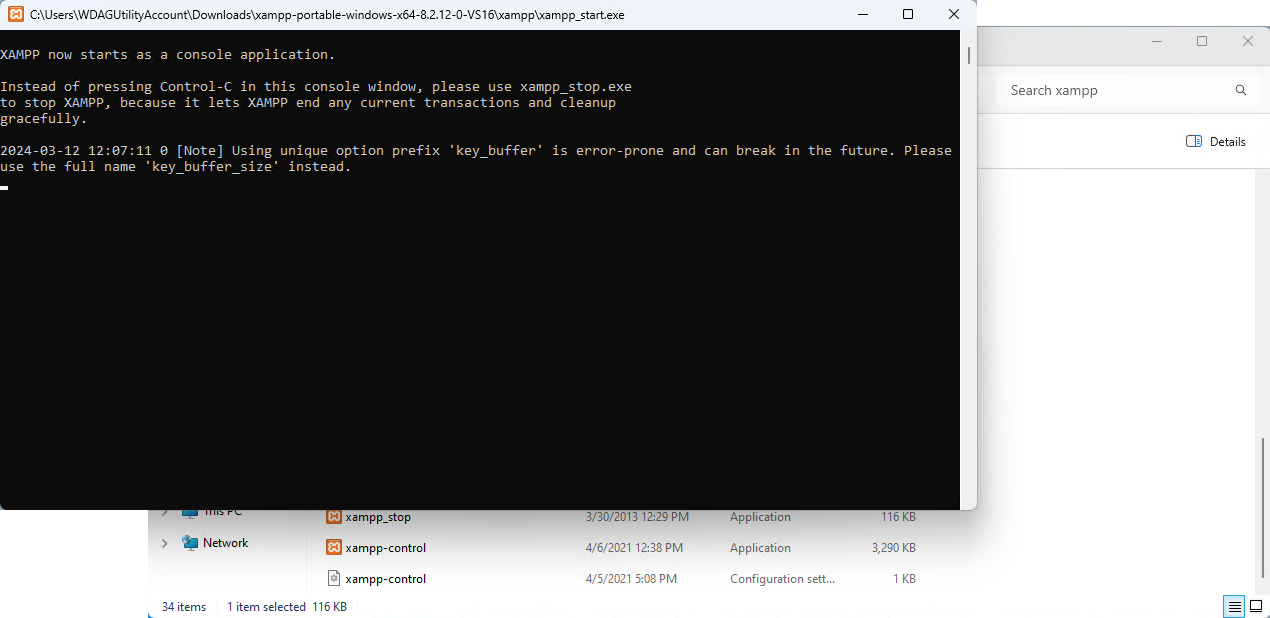
\includegraphics[scale=0.3]{install_xampp13} \\

            Pick a language for the program.                                & 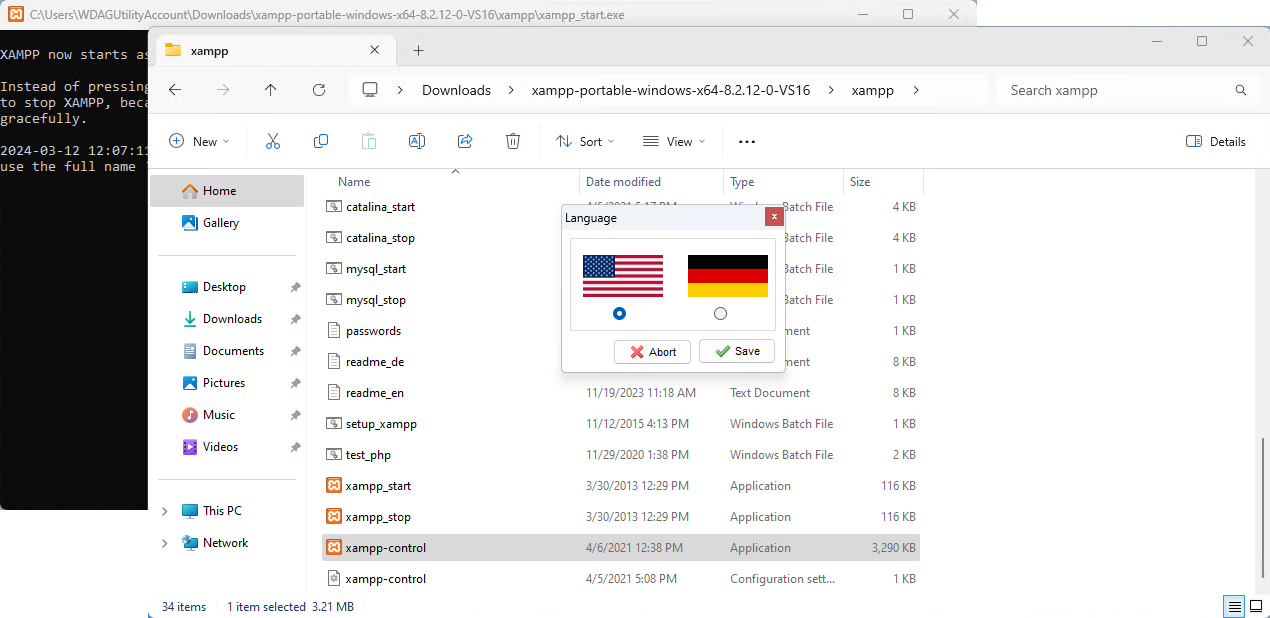
\includegraphics[scale=0.3]{install_xampp14} \\

            Apache2 comes with SSL on by default. Since we're studying the
            HTTP protocol it's convenient to disable HTTPS.
            Pressing the \textit{config} button shows a list of
            configuration files. Select \textit{Apache (httpd-ssl.conf)}.   & 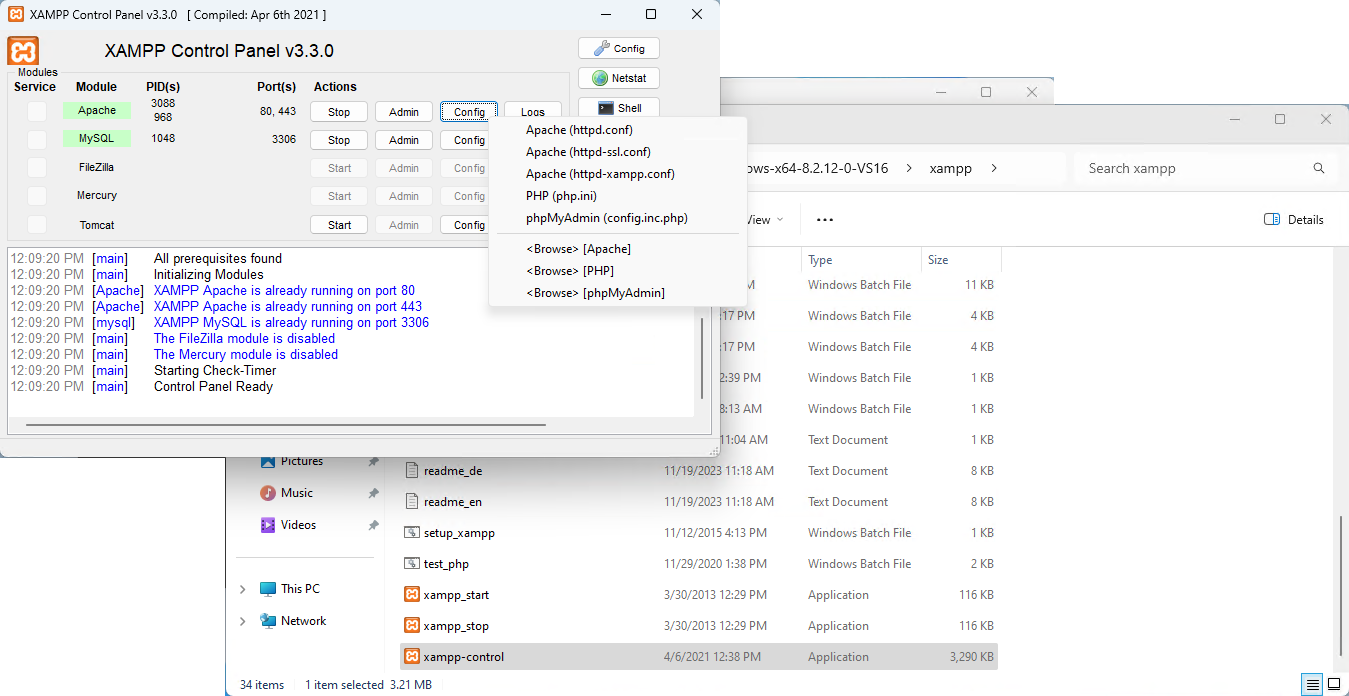
\includegraphics[scale=0.3]{install_xampp15} \\

            Search and comment the line with \textit{SSLEngine on}.         & 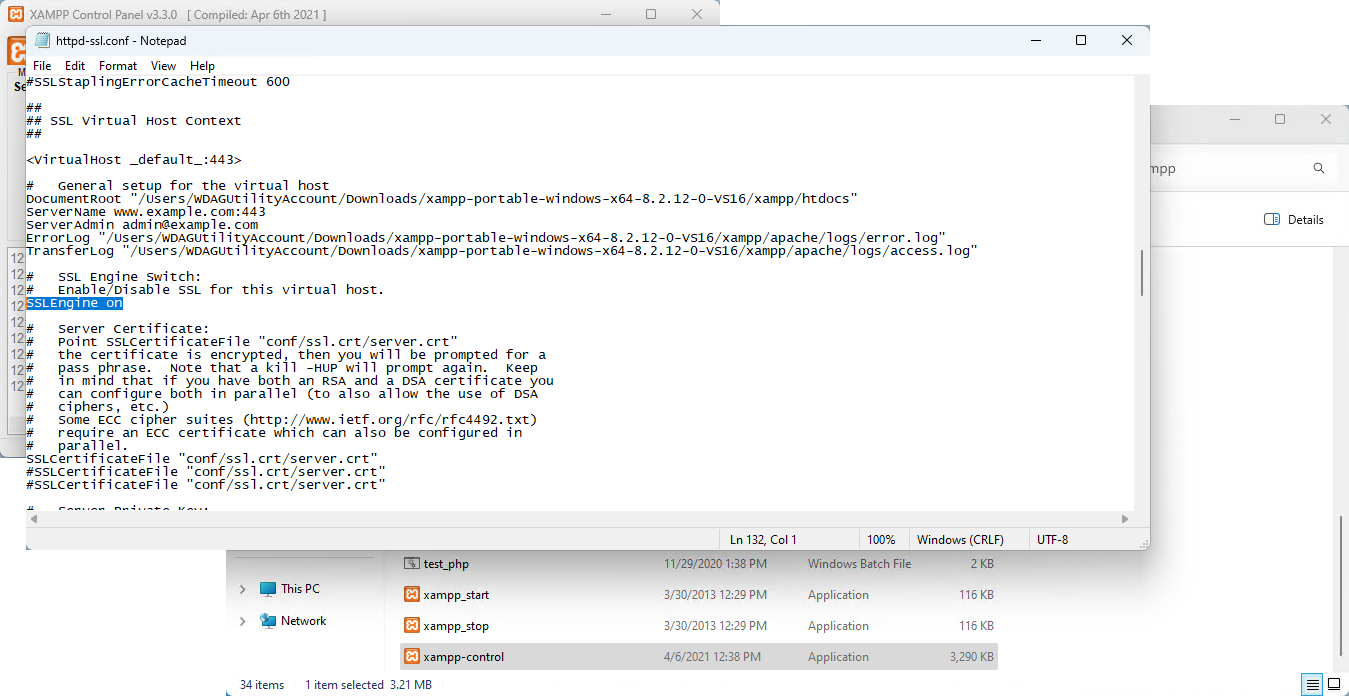
\includegraphics[scale=0.3]{install_xampp16} \\

            Previously if we went to http://localhost it would redirect
            to the HTTPS version. After completing the above step it'll no
            longer redirect, showing us the non-secure version.             & 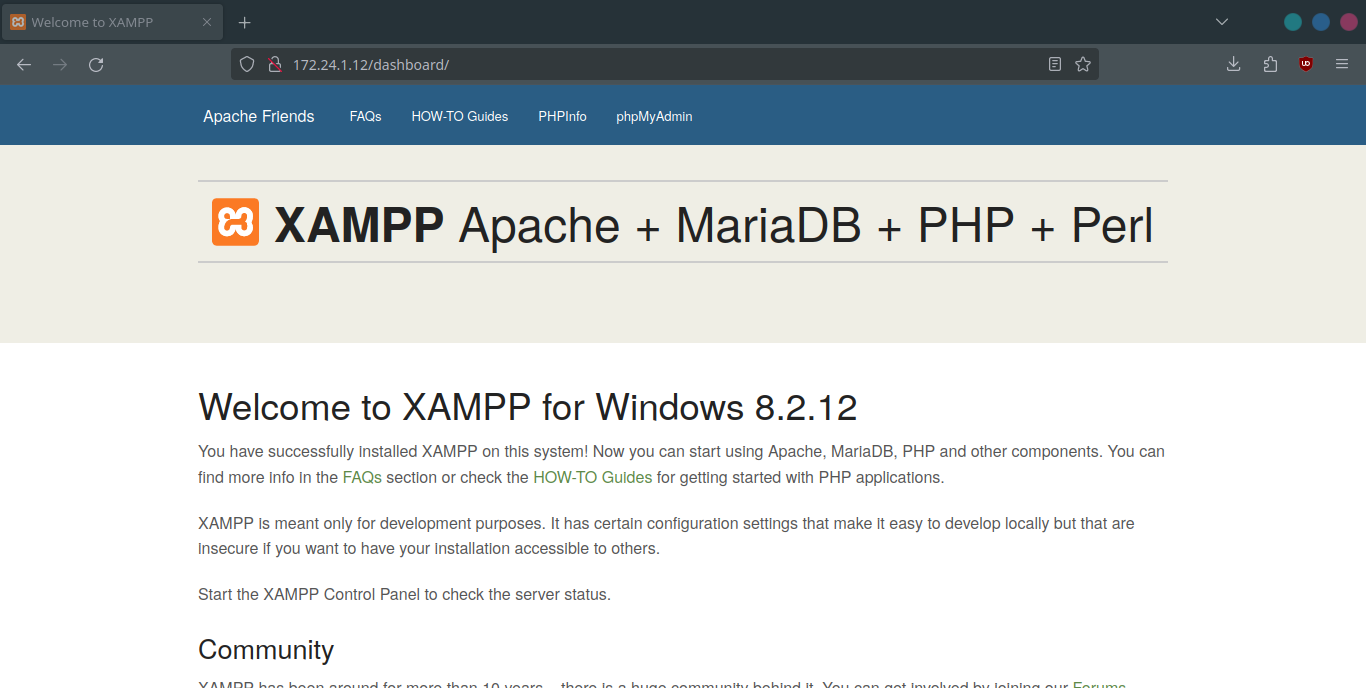
\includegraphics[scale=0.3]{install_xampp17} \\
        \end{tabular}

        % Sério, alterar palavreado!
        Next up is wireshark, the almighty powerful network analyser.
        We shall download the installer, \url{https://www.wireshark.org/download.html}{link} just because it'll be useful for the rest of this semester.
        The install process is pretty simple, selecting everything available and pressing next all the time.
        \begin{tabular}{ l r }
            text & 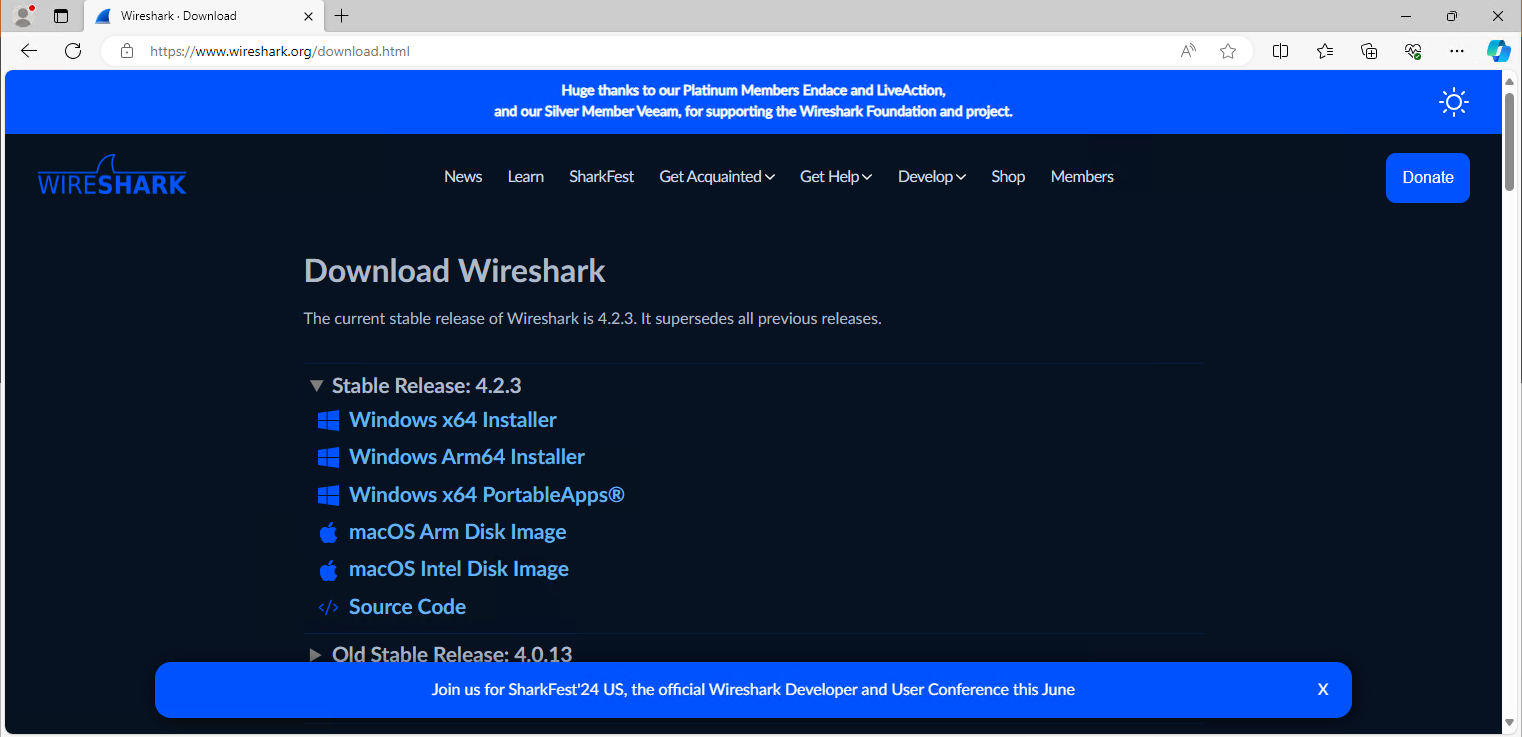
\includegraphics[scale=0.3]{install_wireshark01} \\
            text & 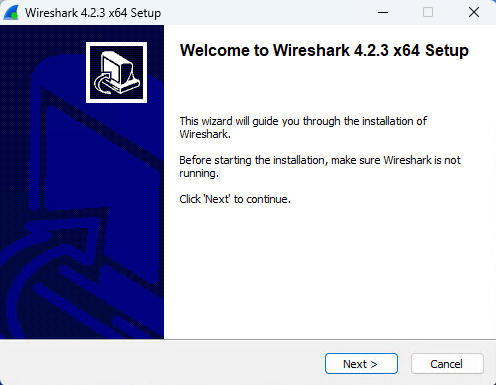
\includegraphics[scale=0.3]{install_wireshark02} \\
            text & 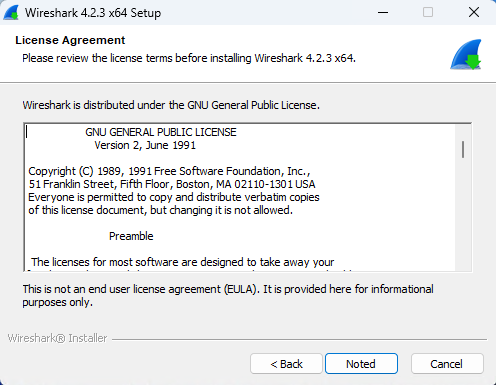
\includegraphics[scale=0.3]{install_wireshark03} \\
            text & 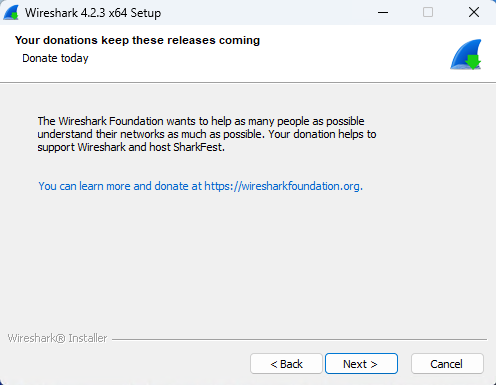
\includegraphics[scale=0.3]{install_wireshark04} \\
            text & 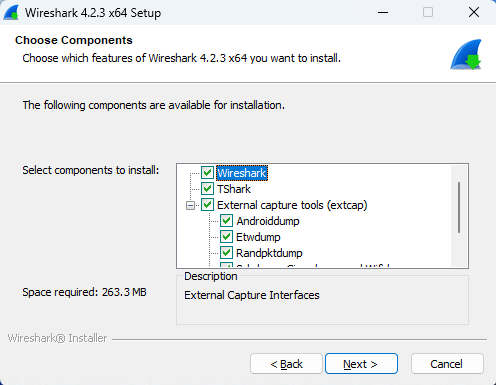
\includegraphics[scale=0.3]{install_wireshark05} \\
            text & 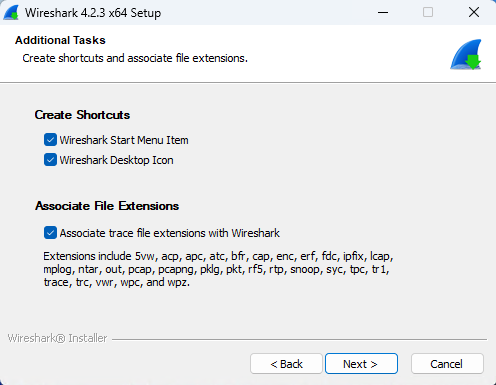
\includegraphics[scale=0.3]{install_wireshark06} \\
            text & 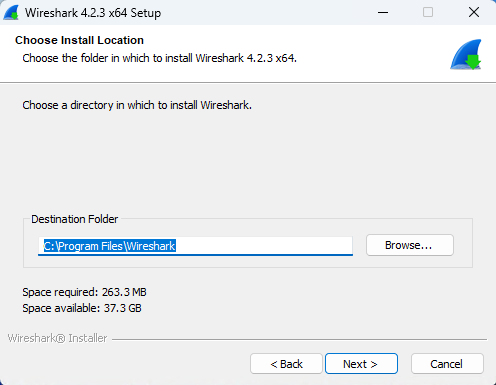
\includegraphics[scale=0.3]{install_wireshark07} \\
            text & 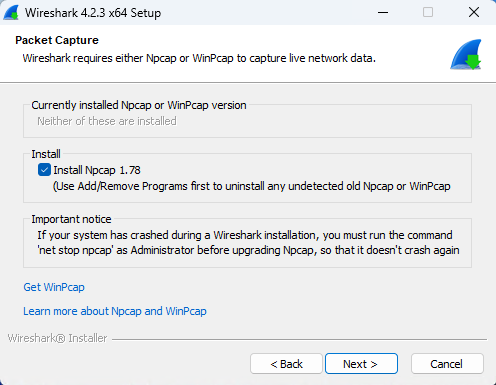
\includegraphics[scale=0.3]{install_wireshark08} \\
            text & 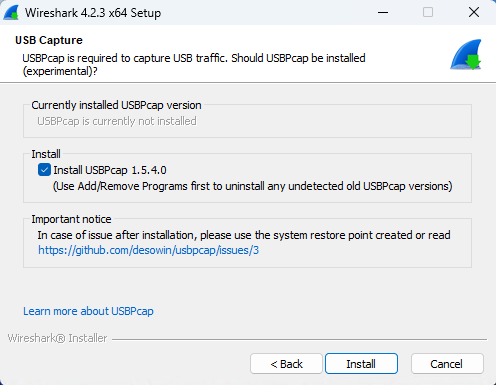
\includegraphics[scale=0.3]{install_wireshark09} \\
            text & 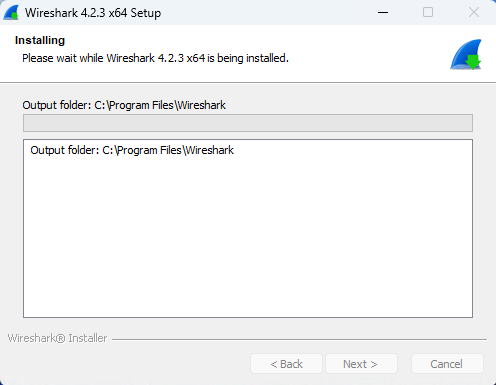
\includegraphics[scale=0.3]{install_wireshark10} \\
            text & 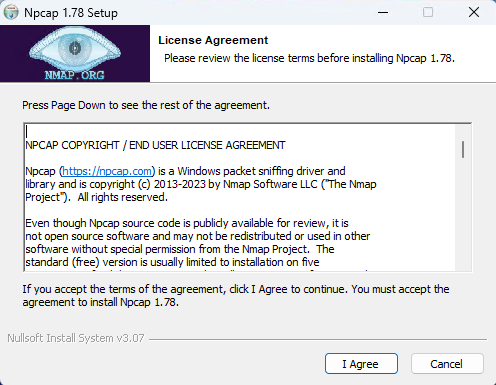
\includegraphics[scale=0.3]{install_wireshark11} \\
            text & 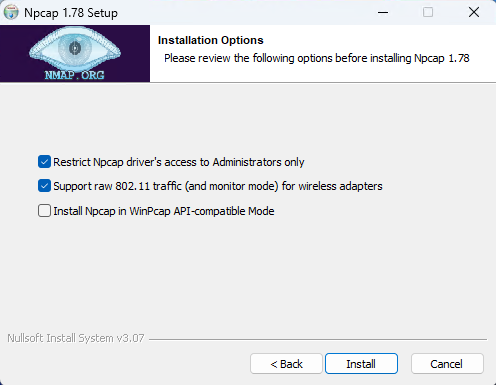
\includegraphics[scale=0.3]{install_wireshark12} \\
            text & 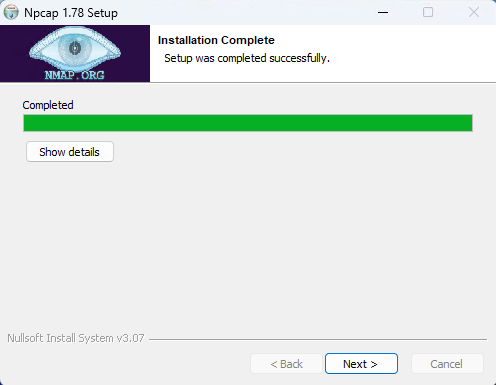
\includegraphics[scale=0.3]{install_wireshark13} \\
            text & 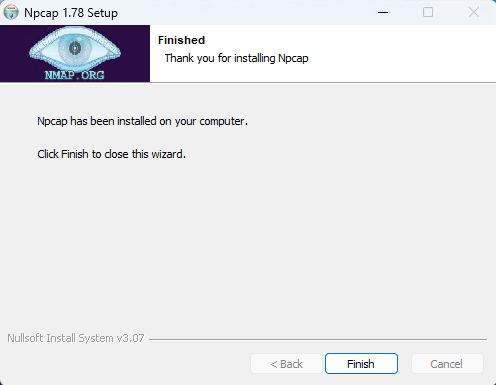
\includegraphics[scale=0.3]{install_wireshark14} \\
            text & 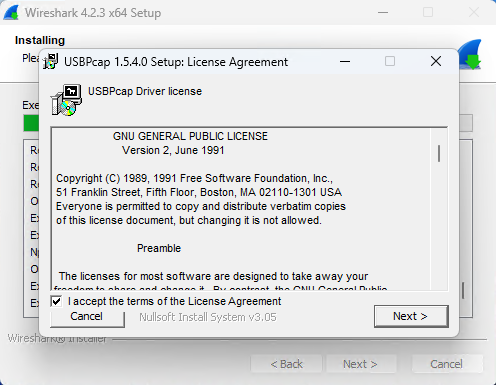
\includegraphics[scale=0.3]{install_wireshark15} \\
            text & 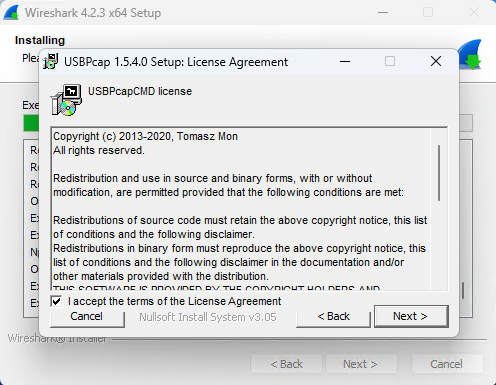
\includegraphics[scale=0.3]{install_wireshark16} \\
            text & 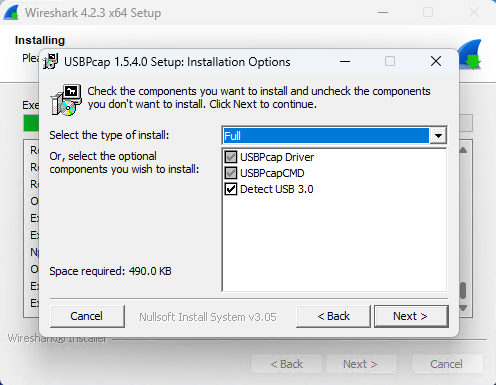
\includegraphics[scale=0.3]{install_wireshark17} \\
            text & 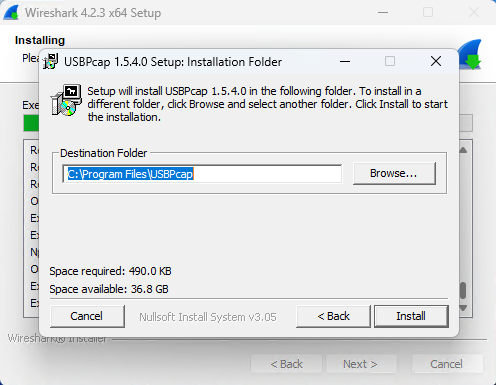
\includegraphics[scale=0.3]{install_wireshark18} \\
            text & 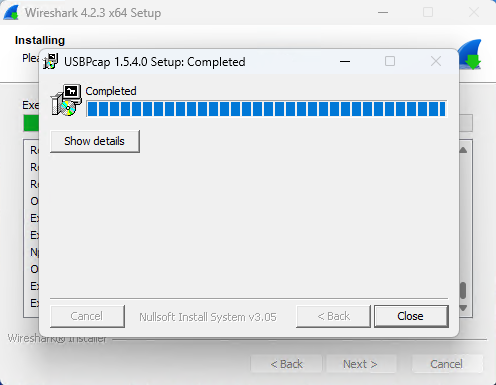
\includegraphics[scale=0.3]{install_wireshark19} \\
            text & 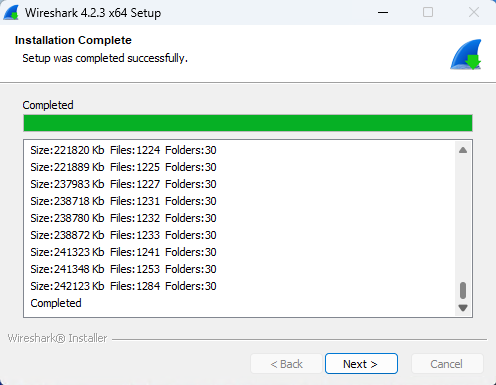
\includegraphics[scale=0.3]{install_wireshark20} \\
            text & 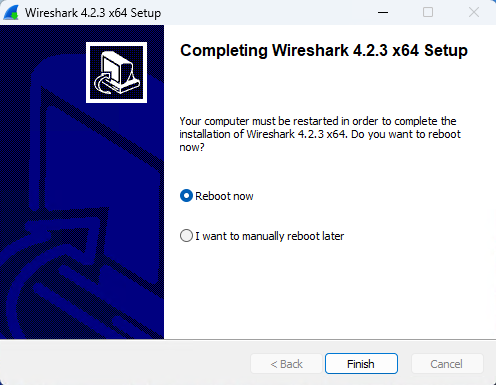
\includegraphics[scale=0.3]{install_wireshark21} \\
        \end{tabular}

    \subsection{WebClient - Python Code}
        \lstset{style=pythoncode}
        \lstinputlisting[language=python, caption=Simple HTTP WebClient using sockets in python]{webclient/httpsocketv3.py}
        The code was adapted to be simple and cycle through the various request messages without any user input.
        Modifiable variables include serverName, serverPort and the httpTestMessages list.

        \VerbatimInput{./webclient/httpsocketv3_output.txt}
        \VerbatimInput{./wireshark/ws_capture01_export.txt}
        \VerbatimInput{./wireshark/ws_capture02_export.txt}
        \VerbatimInput{./wireshark/ws_capture03_export.txt}
    
    \subsection{List of headers and replies}
            \textbf{Request:} GET /dashboard/ HTTP/1.1\r\nHost:127.24.1.12\r\n\r\n
            \textbf{Reply:} HTTP/1.1 200 OK
                Meaning: this header complies with what the server expects from a webclient request.
            \textbf{Request:} GET /dashboard HTTP/1.1\r\nHost:127.24.1.12\r\n\r\n
            \textbf{Reply:} HTTP/1.1 301 Moved Permanently
                Meaning: this header request a relative directory without a forward slash at the end, prompting the server to reply with a "moved" answer.
            \textbf{Request:} PUT / HTTP/1.1\r\nHost:127.24.1.12\r\n\r\n
            \textbf{Reply:} HTTP/1.1 302 Found
                Meaning: this header request is an upload request to an unexistent directory.
            \textbf{Request:} GET /dashboard HTTP/1.\r\nHost:127.24.1.12\r\n\r\n
            \textbf{Reply:} HTTP/1.1 400 Bad Request
                Meaning: this header request, although it has an invalid directory, has the HTTP protocol version badly writen (HTTP/1.1 vs. actual HTTP/1.) which causes
                a "bad request" reply from the server.
            \textbf{Request:} GET /dashboard/index.htm HTTP/1.1\r\nHost:127.24.1.12\r\n\r\n
            \textbf{Reply:} HTTP/1.1 404 Not Found
                Meaning: this header request tries to get a file that doesn't exist in the local server.
            \textbf{Request:} PUT /d HTTP/1.1\r\nHost:127.24.1.12\r\n\r\n
            \textbf{Reply:} HTTP/1.1 405 Method Not Allowed
                Meaning: this header request tries to upload something to the relative directory "d".

    \subsection{Configurations}
        LibreWolf using deprecated TLS and unsecured sites enabled
        SSLEngine disabled in apache2 to ease access with http protocol
        %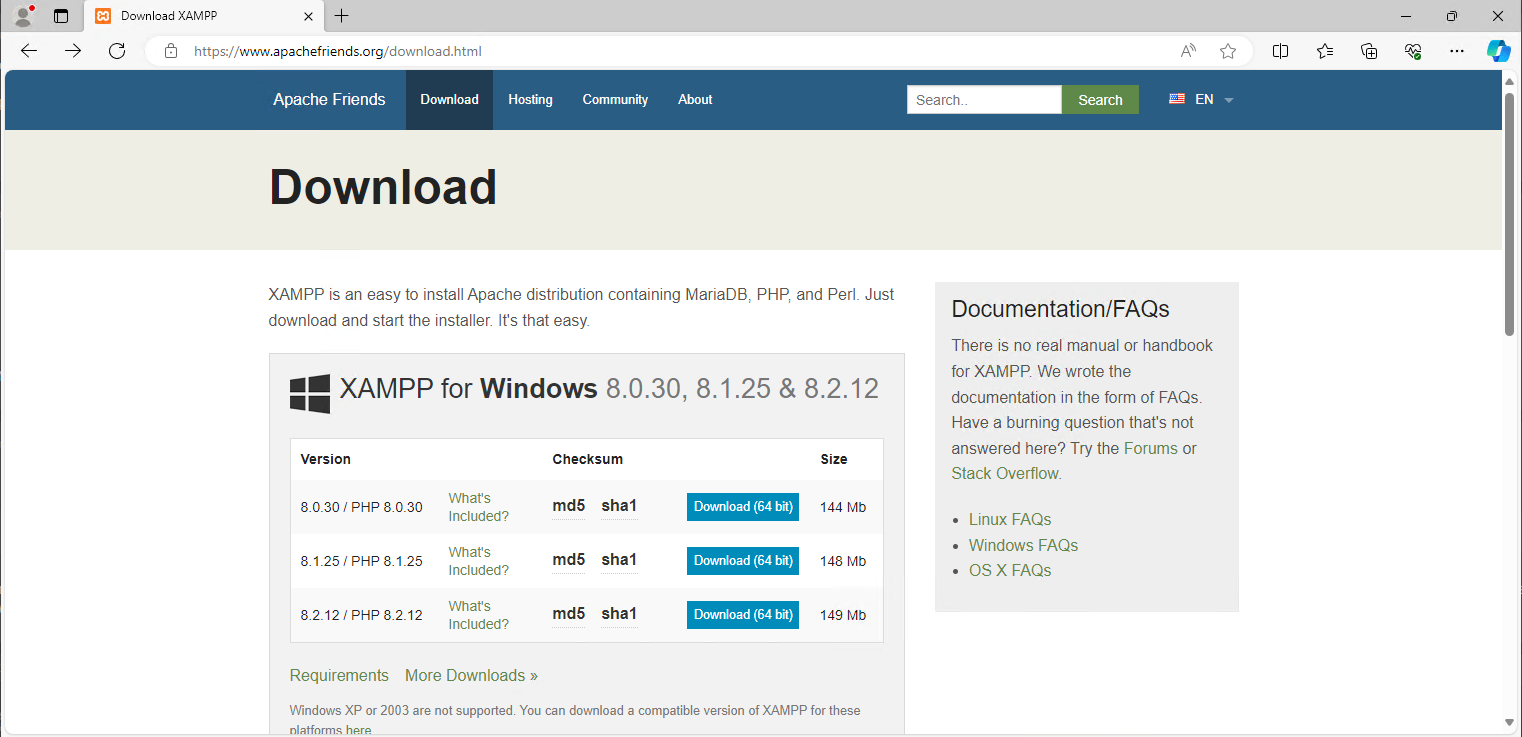
\includegraphics[scale=1.0]{xampp01} \\
        %<=++figure sslengine off++=>
        %<=++figure access from localhost++=>
        %<=++figure access from 127.0.0.1++=>
        %<=++figure access from anotherhost++=>
        %<=++figure wireshark capture from another host++=>
        
        \begin{multicols}{2}
        [Install]
        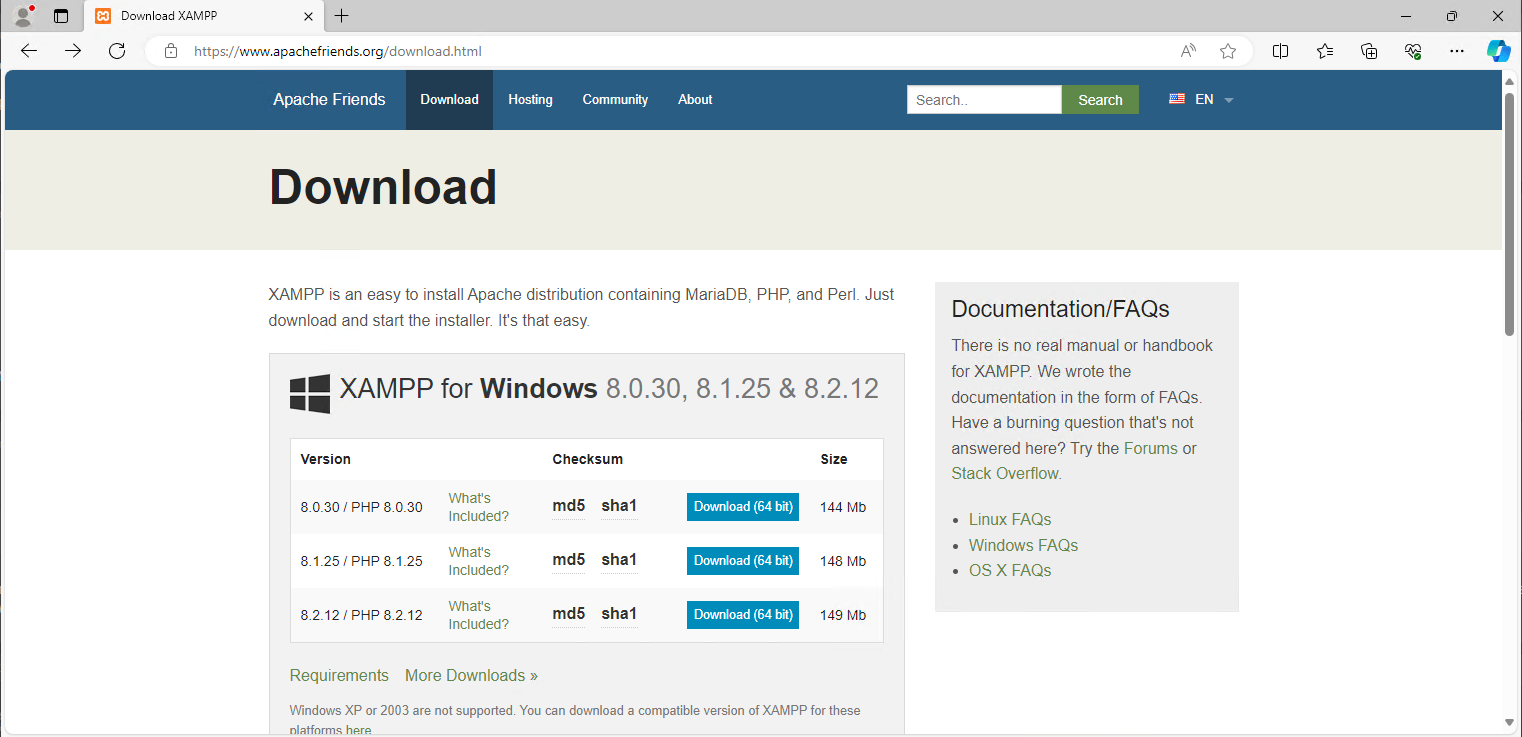
\includegraphics[scale=1.0]{1}

%% Chapter: recomendations -----------------------------------------------------{{{1
\section{Problems and resolutions}
    Python code: default system came with python2. Python3 installed.
    Encrypted html body: since the xampp server is running in a laptop at home and to make some progress i have to work remotely via vpn, the content came encrypted.
    Default http protocol SSL: disabled in apache2 the ssl engine

%% Chapter: conclusions --------------------------------------------------------{{{1

%% Bibliography ----------------------------------------------------------------{{{1
\renewcommand{\bibname}{Referências bibliográficas}
\bibliographystyle{chicago}
\bibliography{refs}
\addcontentsline{toc}{chapter}{\refname}  % add it to table of contents

%% Appendix --------------------------------------------------------------------{{{1
\appendix
\chapter{Um Apêndice}
%%1}}}

\end{document}
